%-------------------------------------------------------------------------------
% File: architecture.tex
%
% Author: Marco Pinna
%         Created on 14/07/2022
%-------------------------------------------------------------------------------
\chapter{Architecture}\label{ch:architecture}
This chapter analyses in greater detail the architecture of the application, showing which modules are present where and how they interact with each other. In the second part the structure of the packets exchanged between modules is presented.
\hfill \break


When a voter enters the polling station, the personnel in charge authenticates them via face recognition and personal documents. After checking that the voter is registered to that polling station, they are allowed to enter the polling booth.\\ The voter authenticates themselves again inside the voting booth with an electronic document, such as an electronic identity card. On each polling booth there is a Tomcat instance running, which will serve the web page on which the voter will express their vote.\\
The voters' electronic document will also contain the private key of the voter ($Priv_{vot\_i}$), which will be used to sign the packet containing the vote; the packet signature will be verified on the polling station upon reception with the corresponding voter's public key ($Pub_{vot\_i}$) contained in the \textit{voter} database, to guarantee authenticity and integrity of the vote.\\
The vote, before being sent over the local network to the polling station server, is encrypted with the public key of the central station ($Pub_{CS}$). The polling station, therefore, is not able to decrypt the vote cast by the voter, and vote secrecy is thus ensured.\\
Once the polling station receives the voter's vote, it sets their corresponding flag \texttt{has\_voted} in the \textit{voter} database to \texttt{true}, to prevent double voting. At this point, the polling station node ``splits" the voter id from the vote and only sends the latter, after signing it with its own private key ($Priv_{PS\_j}$). This ensures the unlinkability of the vote.\\
The central station receives the packet containing the vote, signed by the polling station, and verifies said signature using the corresponding polling station public key ($Pub_{PS\_j}$) which is contained in the \textit{pollingStation} database.\\
Lastly, the vote is saved in the \textit{votes} database in encrypted form. When the voting is over (and only then), the votes will be retrieved from the database and decrypted.

\begin{figure}[H]
    \begin{center}
        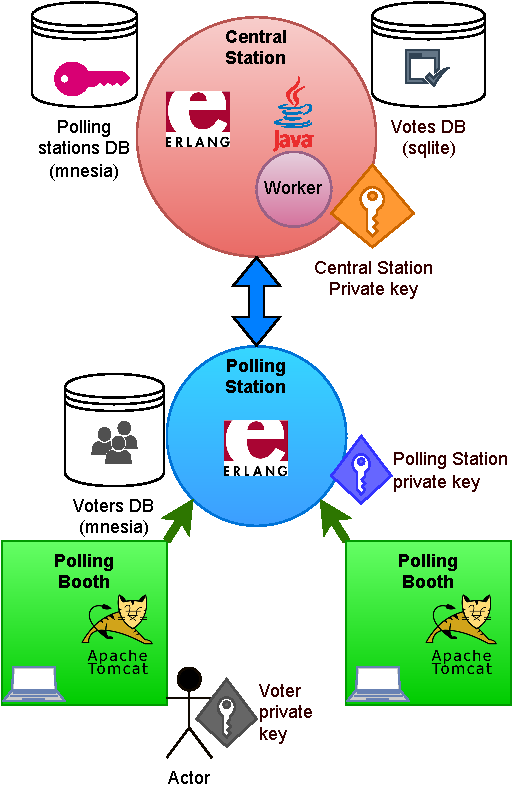
\includegraphics[scale=1]{img/arch_detail.pdf}
    \end{center}
    \vspace*{-0.5cm}
    \caption{A more detailed view of the application architecture.}
    \label{fig:arch_detail}
\end{figure}

\section{Packets structure}